\documentclass{article}

\usepackage{graphicx}
\usepackage{tikz}
\usepackage{tikzsymbols}
\usetikzlibrary{calc,patterns,shapes.geometric}
\pagestyle{empty}
\usepackage[margin=0pt]{geometry}
\geometry{papersize={14in,12in}}

\def\centerarc[#1](#2)(#3:#4:#5){\draw[#1] ($(#2)+({#5*cos(#3)},{#5*sin(#3)})$) arc (#3:#4:#5);}

\begin{document}
	\begin{figure}
		\centering
		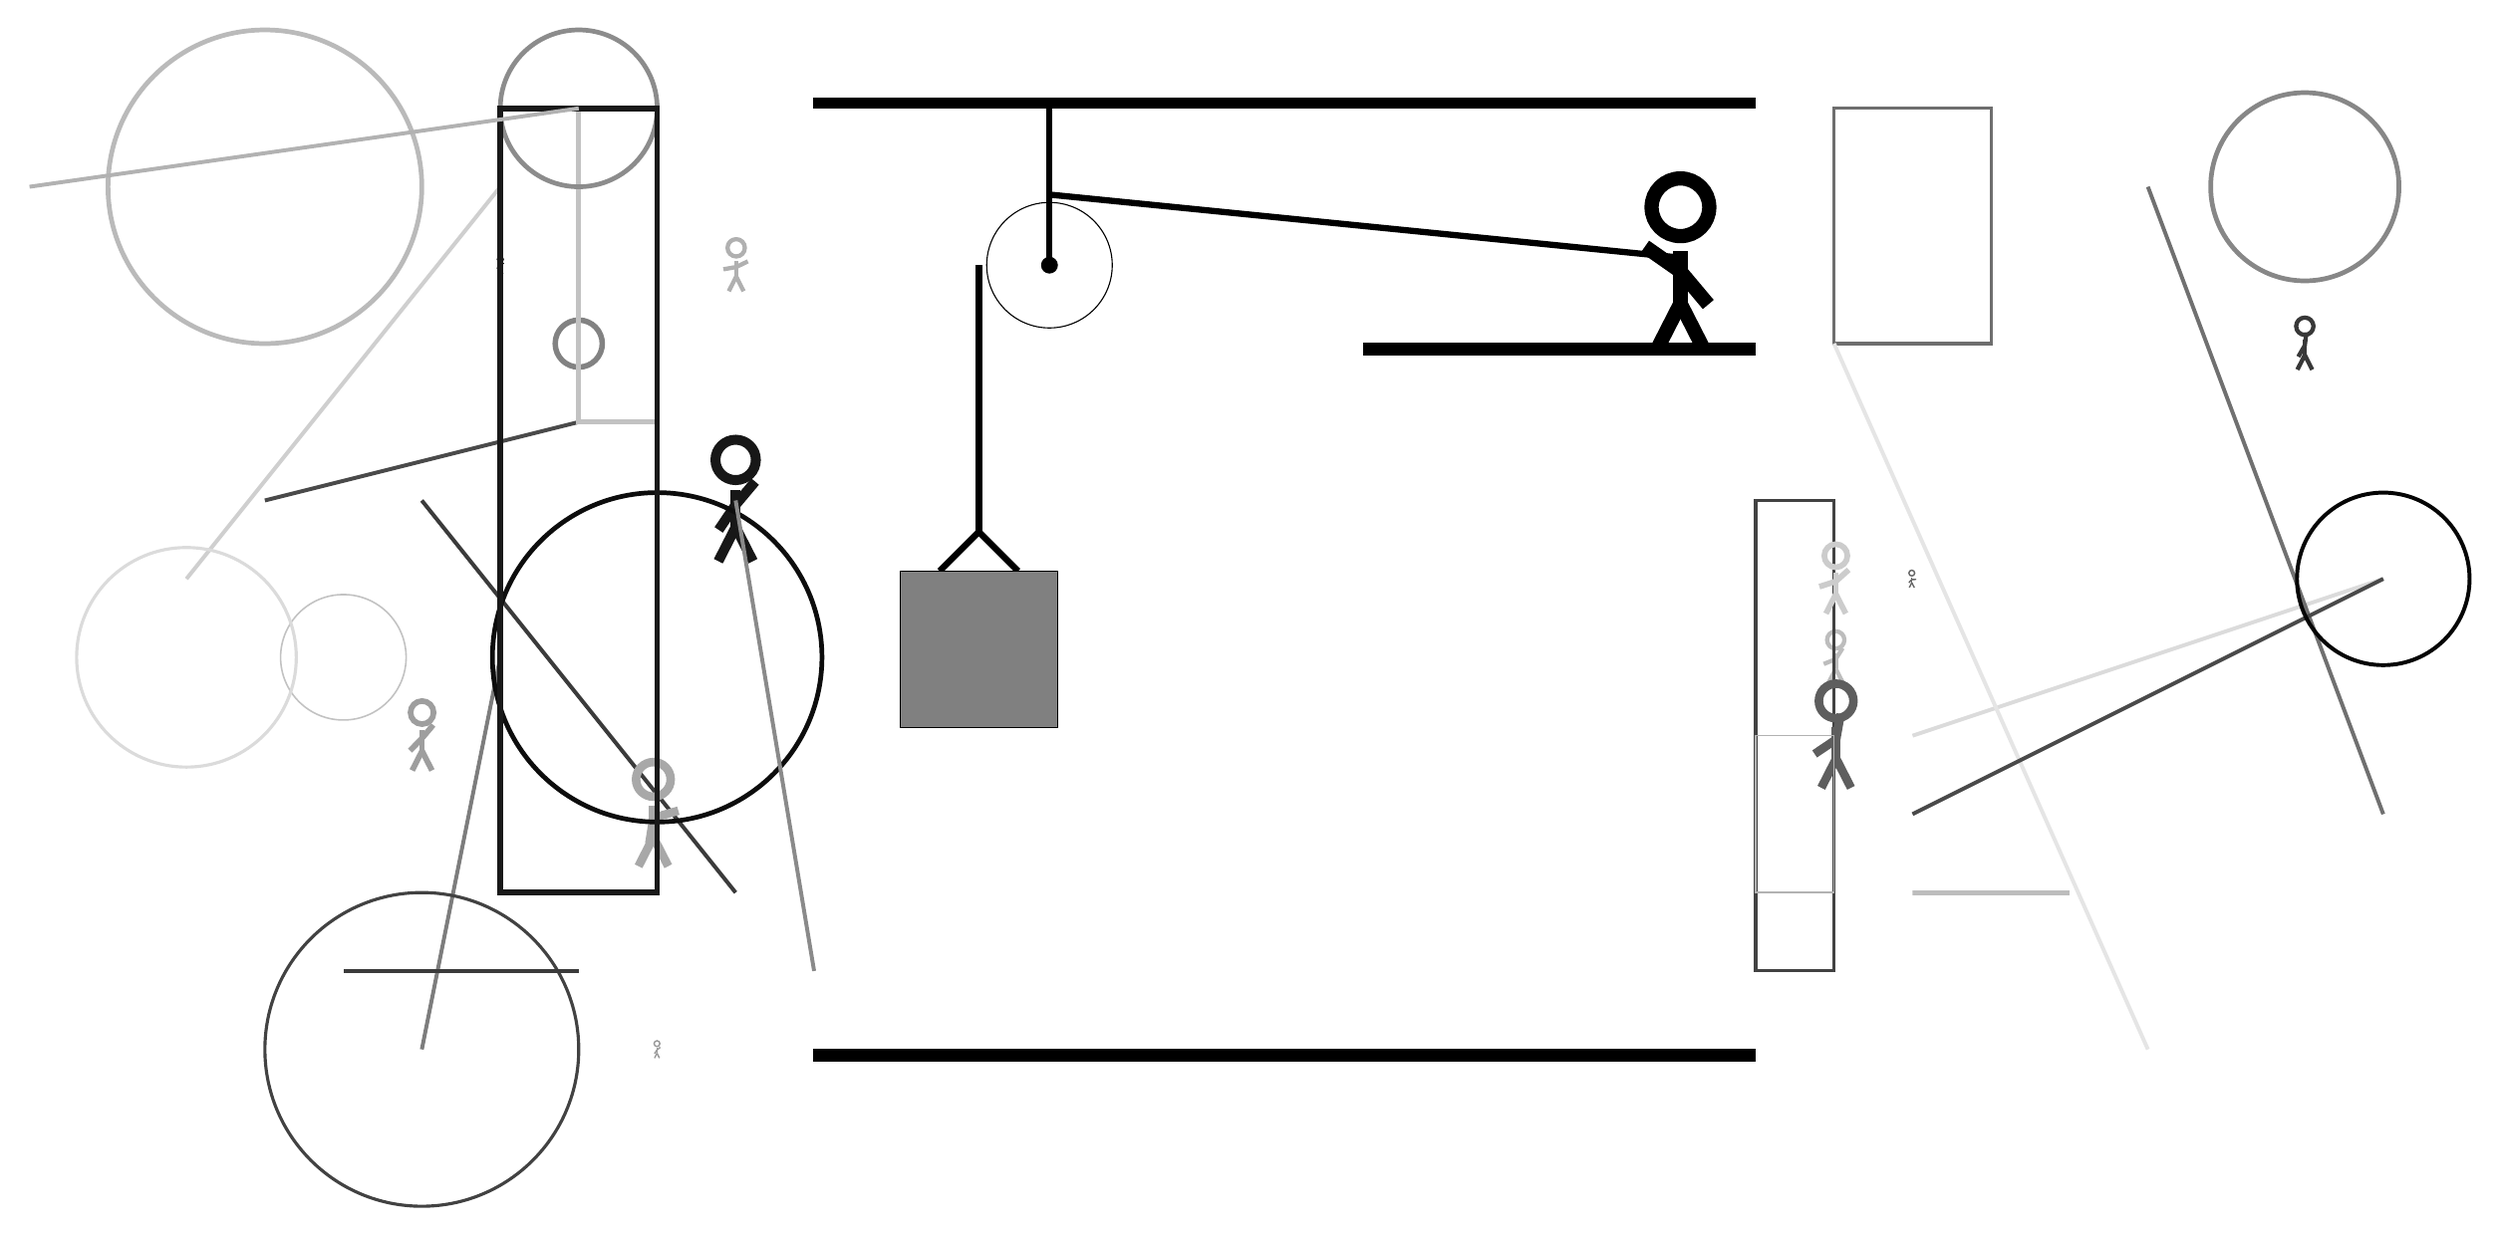
\begin{tikzpicture}
			%%%%% START %%%%%
			
			\draw[fill=black] (-2, 9) rectangle (10, 9.125);
			
			\draw (1, 7) circle (0.8);
			\draw[fill=black] (1, 7) circle (0.1);
			\draw[line width=0.8mm] (1, 9) -- (1, 7);
			
			\draw[line width=0.8mm](-0.4, 3.1) --  (0.1, 3.6) -- (0.6, 3.1);
			\draw[fill=black!50] (-0.9, 3.1) rectangle (1.1, 1.1);
			
			\draw[line width=0.8mm](0.1, 7) -- (0.1, 3.6);
			\centerarc[line width=0.8mm](1, 7)(90:180:0.9)
			\draw[line width=0.8mm](1, 7.9) -- (9, 7.1);
			
			\node at (9, 7) {\Strichmaxerl[10][-35][-50]};
			\draw[fill=black] (5, 6) rectangle (10, 5.85);
			
			\node[line width=0.4mm, color=black!31] at (-3, 7) {\Strichmaxerl[3][10][26]};
			
			\draw[line width=0.5mm, color=black!77](-3, -1) -- (-7, 4);
			\node[line width=0.2mm, color=black!26] at (11, 2) {\Strichmaxerl[3][22][58]};
			\draw [line width=0.7mm, color=black!49](-5, 6) circle (0.3);
			\node[line width=0.5mm, color=black!91] at (-3, 4) {\Strichmaxerl[7][56][50]};
			\draw[line width=0.5mm, color=black!14](12, 1) -- (18, 3);
			\draw[line width=0.4mm, color=black!57] (11, 9) rectangle (13, 6);
			\draw[line width=0.5mm, color=black!71](-5, 5) -- (-9, 4);
			\draw[line width=0.6mm, color=black!24] (-4, 9) rectangle (-5, 5);
			
			\node[line width=0.6mm, color=black!38] at (-7, 1) {\Strichmaxerl[4][46][50]};
			
			\draw[line width=0.5mm, color=black!51](-7, -3) -- (-6, 2);
			
			\draw[line width=0.5mm, color=black!10](11, 6) -- (15, -3);
			\node[line width=0.5mm, color=black!34] at (-4, 0) {\Strichmaxerl[6][81][16]};
			
			\draw [line width=0.4mm, color=black!74](-7, -3) circle (2.0);
			\node[line width=0.4mm, color=black!40] at (-4, -3) {\Strichmaxerl[1][55][40]};
			\draw [line width=0.6mm, color=black!27](-9, 8) circle (2.0);
			
			\draw[line width=0.6mm, color=black!26] (12, -1) rectangle (14, -1);
			\draw[line width=0.4mm, color=black!74] (10, 4) rectangle (11, -2);
			\draw[line width=0.5mm, color=black!77](-5, -2) -- (-8, -2);
			\draw [line width=0.6mm, color=black!95](-4, 2) circle (2.1);
			\draw [line width=0.6mm, color=black!45](-5, 9) circle (1.0);
			
			\node[line width=0.4mm, color=black!60] at (12, 3) {\Strichmaxerl[1][48][1]};
			
			\draw [line width=0.2mm, color=black!24](-8, 2) circle (0.8);
			\draw[line width=0.5mm, color=black!56](15, 8) -- (18, 0);
			\node[line width=0.2mm, color=black!63] at (11, 1) {\Strichmaxerl[6][34][80]};
			
			\draw[line width=0.5mm, color=black!71](12, 0) -- (18, 3);
			\node[line width=0.2mm, color=black!78] at (17, 6) {\Strichmaxerl[3][60][83]};
			\draw [line width=0.5mm, color=black!98](18, 3) circle (1.1);
			\node[line width=0.7mm, color=black!98] at (-6, 7) {\Strichmaxerl[1][38][40]};
			
			\draw [line width=0.6mm, color=black!47](17, 8) circle (1.2);
			\draw[line width=0.5mm, color=black!19](-6, 8) -- (-10, 3);
			\draw [line width=0.4mm, color=black!14](-10, 2) circle (1.4);
			\draw[line width=0.7mm, color=black!90] (-4, 9) rectangle (-6, -1);
			\draw[line width=0.5mm, color=black!30](-5, 9) -- (-12, 8);
			\node[line width=0.7mm, color=black!20] at (11, 3) {\Strichmaxerl[4][18][42]};
			\draw[line width=0.2mm, color=black!30] (10, 1) rectangle (11, -1);
			\draw[line width=0.5mm, color=black!46](-2, -2) -- (-3, 4);
			
			
			\draw[fill=black] (-2, -3) rectangle (10, -3.15);
			
			%%%%% END %%%%%
		\end{tikzpicture}
	\end{figure}	
\end{document}